\section{Решение}
\subsection{Уравнения движения частицы}
По условию задачи мы рассматриваем движение частицы в тороидальном соленоиде,для этой задачи наилучшим образом подходит цилиндрическая система координат:
% \begin{equation*}
%     \begin{cases}
%         \frac{a}{b} \\
%         dd
%     \end{cases}
% \end{equation*}


\begin{equation} 
    \frac{d}{dt}(\gamma m \dot{z}) = q \dot{r} B_{\theta} \label{eq1}
\end{equation}

\begin{equation}
    \frac{1}{r} \frac{d}{dt} (\gamma m r^2 \dot{\theta}) = 0 \label{eq2}   
\end{equation}

\begin{equation}
    \frac{d}{dt}(\gamma m \dot{r}) = \gamma mr \dot{\theta^2} - q \dot{z} B_{\theta}   \label{eq3}
\end{equation}
По условию задачи электрическое поле отсутствует, магнитное поле направлено только азимутально. 
\par
Проинтегрируем по времени уравнения \eqref{eq1} и \eqref{eq2}
\begin{equation}
     \gamma m r^2 \dot{\theta} = L_{\theta} = const
\end{equation}

\begin{equation}
    \gamma m \dot{z} = \int{q \frac{dr}{rdt}B_0 r_0}dt = q B_0 r_0 \ln{r} + C_2
\end{equation}
Третье уравнение можно проинтегрировать только численно. Об этом следующий пункт.
\newpage

\subsection{Численное решение уравнений движения}

Численно проинтегрируем оставшееся уравнение движения \eqref{eq3} для следующих параметров: \(B = 40 \) Гс,  \(r_0 = 1 м\) м, частица – \(e^-\), в начале имеет только азимутальную скорость, начальная энергия \(W = 100 \) кэВ. 

\begin{equation}
    \ddot{r} = r \dot{\theta}^2 - \dot{z} \frac{qB_0 r_0}{m} \frac{1}{r}   
\end{equation}
С учетом того, что $ \dot{\theta} = r_0^2 \dot{\theta}_0 / r^2 $ %где $v_0 = \theta_0 r_0

\begin{equation}
    \ddot{r} = \frac{2W r^2_0}{m r^3} - \dot{z} \frac{qB_0 r_0}{m} \frac{1}{r}    
\end{equation}
Где $ \dot{z} $ :

\begin{equation}
    \dot{z} = \frac{q B_0 r_0}{m} \ln{\frac{r}{r_0}} + \dot{z}_0 \label{dotz}
\end{equation}
Для удобства, переобозначим константы в $\eta_1$ и $\eta_2$.
\begin{equation}
    \ddot{r} =\eta_1 \frac{1}{r^3} - \left(\eta_2\ln{\frac{r}{r_0}} + \dot{z}_0 \right) \eta_2 \frac{1}{r} \label{eq4}
\end{equation}

\begin{equation}
    \eta_1 = \frac{2W r_0^2}{m}
\end{equation}

\begin{equation}
    \eta_2 = \frac{qB_0 r_0}{m}
\end{equation}


Дифференциальное уравнение решим численно с помощью метода Эйлера на языке программирования Python. \par
Из условия задачи следует, что $\dot{z}_0 = 0, r(t=0) = r_0, \dot{r}(t=0) = 0$. Решение уравнения предоставленно в виде графиков на (Рис.~\ref{fig:1}) 
\newpage
\begin{figure}[h]
    \centering
    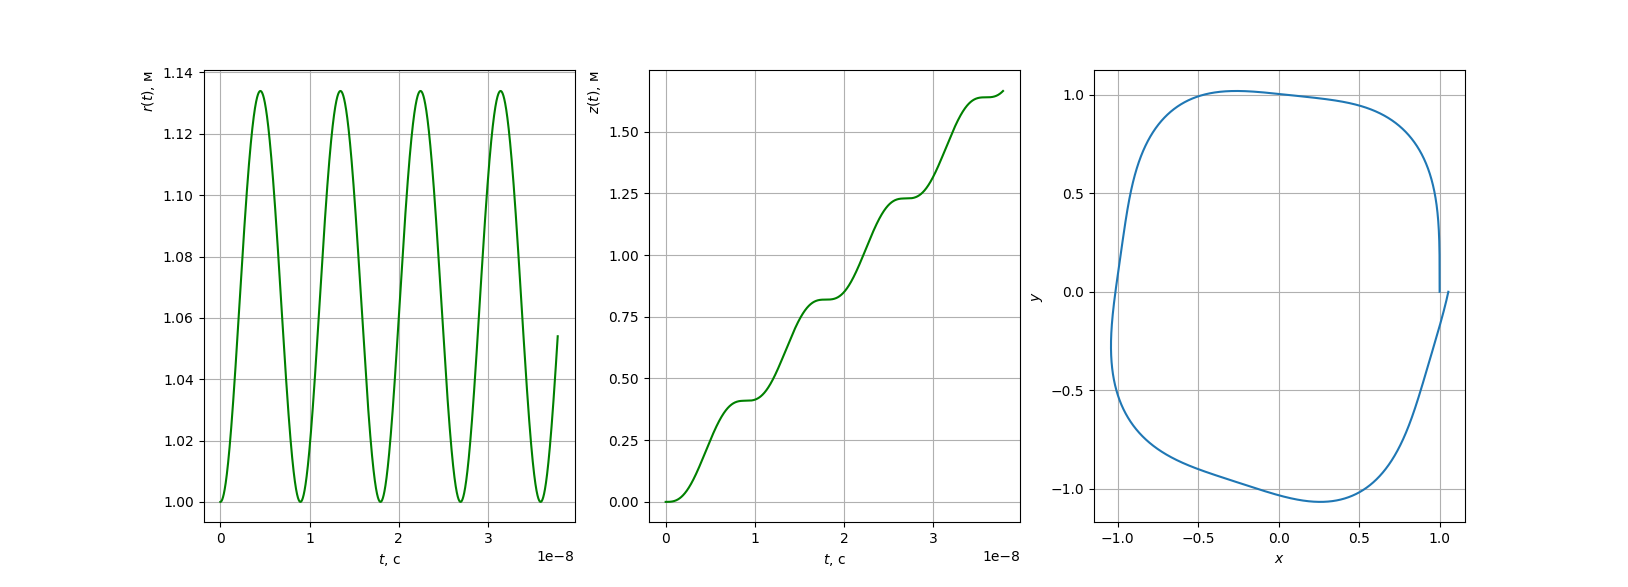
\includegraphics[width=1\linewidth]{../prog/Figure_1.png}\caption{Движение электрона вокруг окружности за 1 период по $r(t)$, $z(t)$, $y(x)$ соответсвенно.}\label{fig:1}
\end{figure}

Период найден численно и равен $T = 3.78 \cdot 10^{-8} c $
\par
Чтобы численное решение связать с дрейфовой теорией, нужно найти $v_{||}$ -- скорость движения ведущего центра вдоль силовой линии магнитного поля.
Скорость центробежного дрейфа равна по определению:
\begin{equation}
    \Vec{v}_{cf} = \frac{\gamma m v_{||}^2}{q} \frac{1}{B^2} \left[\Vec{B}\times \frac{\Vec{n}}{r}\right] \label{6}
\end{equation}
Из уравнения \eqref{6} видно, что вектор скорости центробежного дрейфа будет направлен вдоль оси $z$.
Подставляя скорость $v_{||}$ в уравнение \eqref{6}, получим следующее.
\begin{equation}
   v_{cf}(r) = \frac{2W}{q B_0} \frac{r_0}{r^2}
\end{equation}
Численно решая приведенное уравнение, найдем еe траекторию вдоль оси $z$ (Рис ~\ref{fig:2})
\begin{figure}[h]
    \centering
    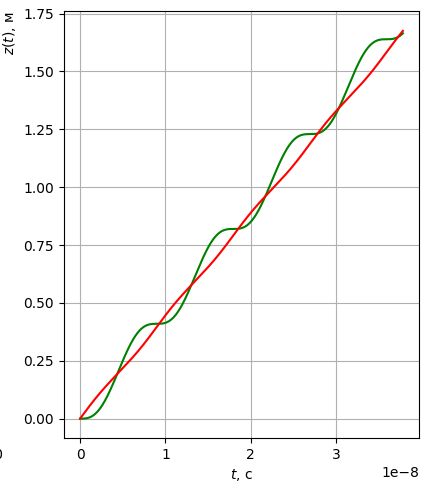
\includegraphics[width=0.3\linewidth]{../prog/screen1.png}\caption{Красной линией помечена траектория дрейфа.}\label{fig:2}
\end{figure}
\newpage
\subsection{Нахождение параметров для постоянного радиуса кривизны траектории электрона}

Частица будет иметь постоянный радиус, при условии, что радиальная скорость $\dot{r} = 0$, следовательно $\ddot{r} = 0$. Тогда уравнение \eqref{eq4} принимает вид:

\begin{equation}
    \frac{2W r^2_0}{m r^3} - \left(\frac{q B_0 r_0}{m} \ln{\frac{r}{r_0}} + \dot{z}_0 \right) \frac{qB_0 r_0}{m} \frac{1}{r} = 0
\end{equation}
При этом, $r(t) = r = r_0$. Решая уравнение, найдем $\dot{z}_0$.
\par
Получим, что $\dot{z}_0 = 5 \cdot 10^{7}$ м/c.
Подставим в  \eqref{eq4}, получим следующие графики (см. ~\ref{fig:2})
\begin{figure}[h]
    \centering
    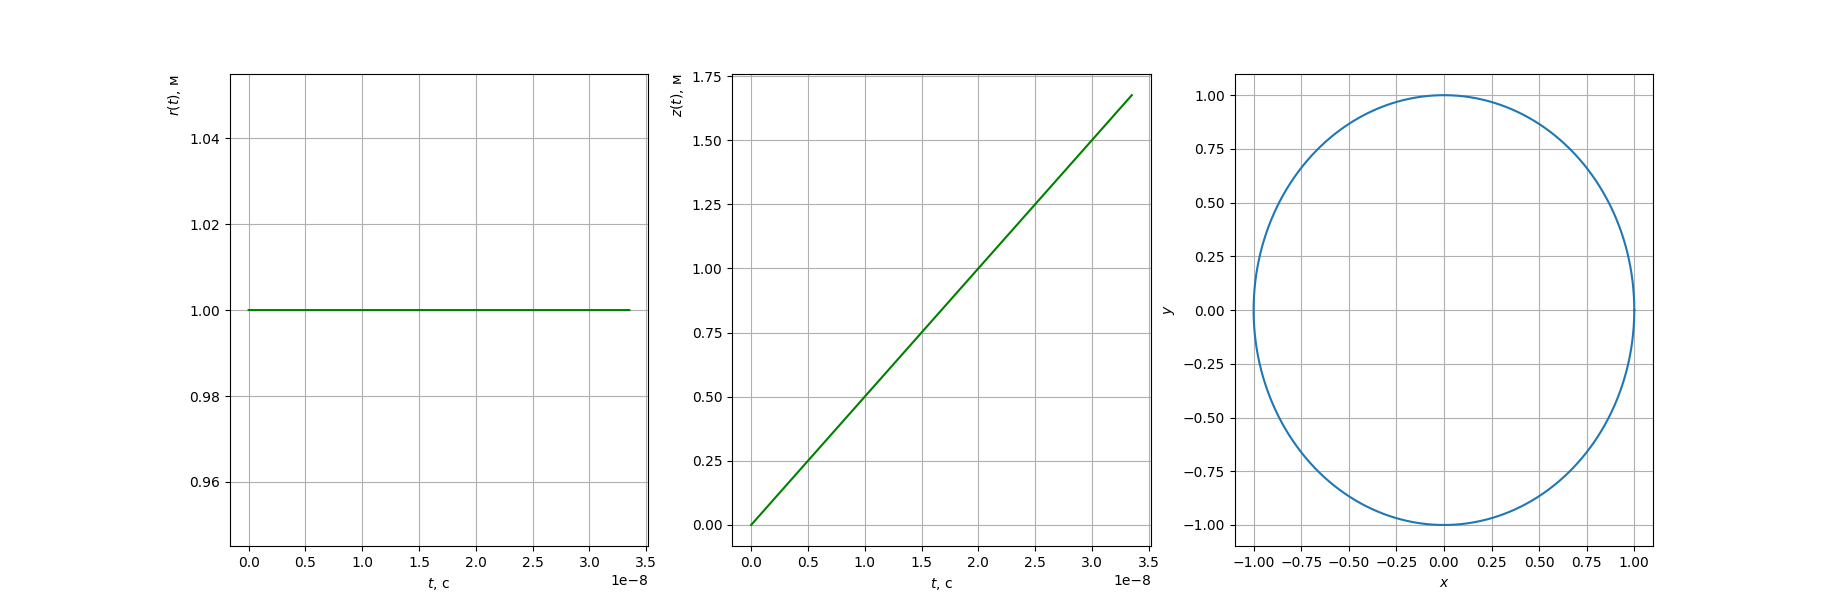
\includegraphics[width=1\linewidth]{../prog/Figure_2.png}\caption{}\label{fig:2}
\end{figure}
\par
Действительно, получилась идеальная окружность. При таких условиях, электрон движется вдоль оси $z$ с постоянной скоростью $\dot{z}(t) = const$.



\newpage
\subsection{Линеаризация уравнений }
Линеаризуем уравнение \eqref{eq1} с помощью ряда Тейлора с теми же условиями (параметрами), при которых искалось численное решение.
\begin{equation}
    \ddot{r}=\eta_1 \frac{1}{r^3} - \eta_2^2 \frac{1}{r} \ln{\frac{r}{r_0}}   
\end{equation}
Преобразуем $r$ в:
\begin{equation}
    r = r_m + \delta(t)    
\end{equation}
Где $r_m$ -- середина синусоиды, ее середину возьмем из численного решения, $\delta(t)$ -- колебания. 

\begin{equation}
    \frac{1}{r^3} \approx \frac{1}{r_m^3} - \frac{3\delta(t)}{r_m^4};   
\end{equation}

\begin{equation}
    \frac{1}{r} \ln{\frac{r}{r_0}} \approx \frac{\ln{\frac{r_m}{r_0}}}{r_m} + \frac{\delta(t) (1 - \ln{{\frac{r_m}{r_0}}})}{r_m^2}   
\end{equation}
Получим дифференциальное уравнение второго порядка:
\begin{equation}
    \ddot{\delta} = \eta_1 \left( \frac{1}{r_m^3} - \frac{3\delta(t)}{r_m^4}\right) - \eta_2^2 \left( \frac{\ln{\frac{r_m}{r_0}}}{r_m} + \frac{\delta(t) (1 - \ln{{\frac{r_m}{r_0}}})}{r_m^2}\right)
\end{equation}
\begin{equation}
    \ddot{\delta} + k^2 \delta = \eta_1 \frac{1}{r_m^3} - \frac{\eta_2^2}{r_m}\ln{\frac{r_m}{r_0}}    
\end{equation}

\begin{equation}
    k^2 = \frac{3\eta_1}{r_m^4} + \frac{\eta_2^2 (1 - \ln{\frac{r_m}{r_0}})}{r_m^2}
\end{equation}

\begin{equation}
    \delta(t) = C_1 \sin{kt} + C_2 \cos{kt} + \left( \eta_1 \frac{1}{r_m^3} - \frac{\eta_2^2}{r_m}\ln{\frac{r_m}{r_0}}    \right)/k^2 
\end{equation}

\begin{equation}
    r(t) = r_m +   C_1 \sin{kt} + C_2 \cos{kt} + \left( \eta_1 \frac{1}{r_m^3} - \frac{\eta_2^2}{r_m}\ln{\frac{r_m}{r_0}}    \right)/k^2   
\end{equation}
Из начальных условий получим значения констант: \(C_1, C_2\)

\begin{equation}
    C_1 = 0    
\end{equation}
\begin{equation}
    C_2 = r_0 - r_m - \left( \eta_1 \frac{1}{r_m^3} - \frac{\eta_2^2}{r_m}\ln{\frac{r_m}{r_0}}    \right)/k^2       
\end{equation}

\begin{equation}
    r(t) = r_m + \left[ r_0 - r_m - \left( \eta_1 \frac{1}{r_m^3} - \frac{\eta_2^2}{r_m}\ln{\frac{r_m}{r_0}}    \right)/k^2    \right] \cos(kt) +    \left( \eta_1 \frac{1}{r_m^3} - \frac{\eta_2^2}{r_m}\ln{\frac{r_m}{r_0}}    \right)/k^2   
\end{equation}

Линеаризуем $\dot{z}$ (ур. \eqref{dotz}) с помощью ряда Тейлора


\begin{equation}
    \dot{z} = \eta_2 \ln{\frac{r}{r_0}} \approx \eta_2 \left(\ln{\frac{r_m}{r_0}} + \frac{\delta(t)}{r_m}  \right)
\end{equation}
\begin{equation}
    z = \int{\eta_2 \left( \ln{\frac{r_m}{r_0}} + \frac{\delta(t)}{r_m}\right)} dt    
\end{equation}
\begin{equation}
    \int{\frac{\delta}{r_m}}dt = \left( \frac{\eta_1}{r_m^3} + \frac{\eta_2^2}{r_m} \ln{\frac{r_m}{r_0}} \right) \frac{t}{k^2 r_m} + \frac{C_2}{k r_m} \sin{kt}    
\end{equation}

\begin{equation}
    z(t) = \eta_2 t \ln{\frac{r_m}{r_0}} + \left( \frac{\eta_1}{r_m^3} + \frac{\eta_2^2}{r_m} \ln{\frac{r_m}{r_0}} \right) \frac{t \eta_2}{k^2 r_m} + \frac{C_2 \eta_2}{k r_m} \sin{kt}    
\end{equation}
Нарисуем графики полученных $r(t)$, $z(t)$,$v_z(t)$ аналитических решение (см. ~\ref{fig:4}) за период $T$.
\begin{figure}[h]
    \centering
    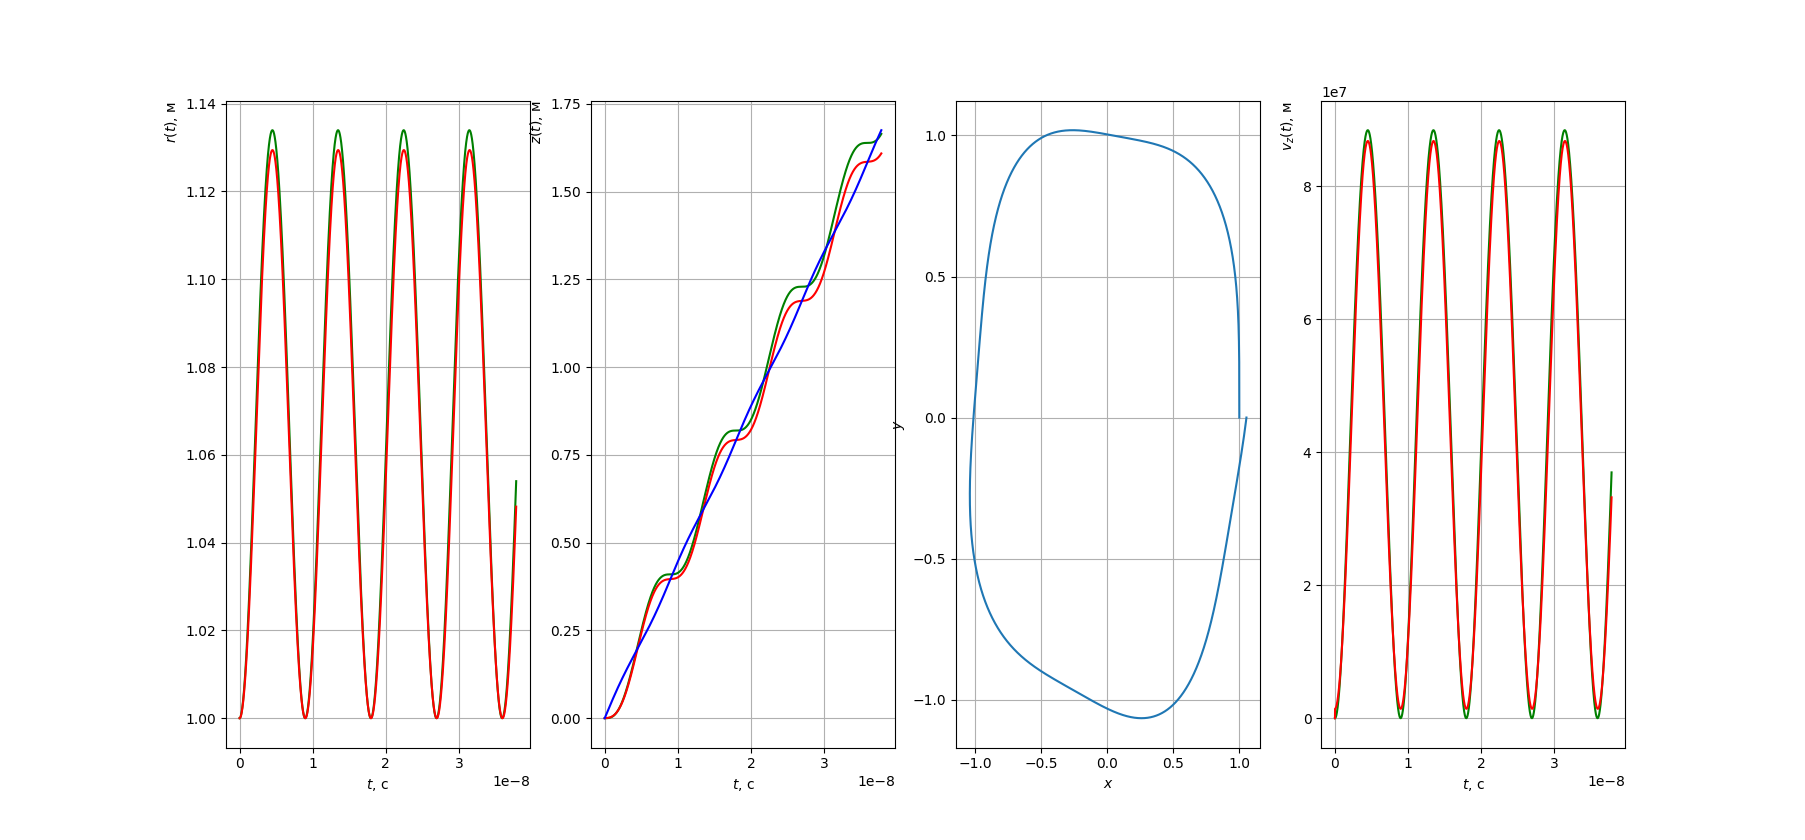
\includegraphics[width=1\linewidth]{../prog/Figure_3.png}\caption{Красной линией обозначено аналитическое решение, зелёным -- численное. }\label{fig:4}
\end{figure}
\par
Видно, что графики аналитического и численного решения разнятся с небольшой погрешностью.
% \lstinputlisting[language=Python]{../prog/main.py}
\newpage
\section{Заключение}
В курсовой работе было подробно описано движение электрона в тороидальном соленоиде с помощью численного метода и аналитического (методом линеаризация). Найдены условия, при которых частица сможет двигаться с постоянным радиусом. 